


\chapter{Arquitectura de instalación}
A la hora de realizar la instalación de un sistema de información, y teniendo en cuenta que es un pilar fundamental de la empresa, habrá que tomar ciertas decisiones desde el punto de vista de sistemas hardware.

De estas decisiones se encargará el \textbf{\textit{sysadmin}}, o administrador de sistemas, pero tendrá que tener ayuda de los especialistas de la aplicación de sistemas de información, así como de determinar una decisión desde el punto de vista empresarial.

Entre las tareas que hay que tener en cuenta, se podrían destacar las siguientes:

\begin{itemize}
    \item \textbf{Hardware}: Determinar el hardware en donde se va a realizar la instalación. Hoy en día existen distintas alternativas, como son:
    \begin{itemize}
        \item \textbf{Hardware dedicado}: Un servidor propio para el sistema, donde se realizará la instalación sólo para este servicio.
        \item \textbf{Máquina Virtual}: El servicio será instalado en una máquina virtual a través de un sistema de virtualización profesional. El servicio es agnóstico al hardware, por lo que no sabrá si está virtualizado o no. Hoy en día suele ser la opción más común dadas las ventajas que ofrecen.
    \end{itemize}

    \item \textbf{Elección del sistema de información}: Esta es una tarea importante y que no se puede dejar de lado, ya que la decisión de optar por una herramienta u otra puede suponer un problema a futuro.

    Es por eso que se debe realizar un estudio de mercado entre las distintas posibilidades y tener en cuenta, al menos, las siguientes situaciones:

    \begin{itemize}
        \item \textbf{Estado actual de la herramienta}: Es importante saber si la herramienta analizada cuenta con un desarrollo continuado, si existe una empresa o grupo de desarrollo por detrás que la apoye; que no esté abandonada; que sea una herramienta con buena aceptación y críticas...
        \item \textbf{Coste de licencia}: Es una herramienta que cuenta con una licencia a perpetuidad bajo un coste determinado\textbf{,} tiene licencia por el número de usuarios que acceden a ella\textbf{,} es una herramienta de Software Libre ...
        \item \textbf{Seguridad, actualizaciones y parches}: La herramienta cuenta con actualizaciones de seguridad periódicas; no ha habido fallos de seguridad graves en las últimas versiones; cuando se detectan fallos las actualizaciones aparecen de manera rápida y efectiva; las actualizaciones y/o parches son gratuitos o de pago...
        \item \textbf{Coste de mantenimiento}: Existe un coste asociado al mantenimiento de la aplicación, pero este puede ser por parte del sistema (realizar actualizaciones, aumento de recursos...) o por pago de licencias anuales, por versiones...
        \item \textbf{Posibilidades de personalización}: Existe la posibilidad de personalizar la herramienta; parametrizar opciones propias que se ajustan a la empresa; creación de módulos/plugins propios para mejorar/expandir la funcionalidad de la herramienta, ...

        \item \textbf{Conocimientos sobre la herramienta}: Dentro de la organización se cuenta con conocimientos acerca del uso/instalación/administración de la herramienta, debe ser subcontratado o existe la posiblidad de adquirir conocimiento mediante cursos o manuales.
    \end{itemize}

    \item \textbf{Sistema operativo}: Dependiendo del sistema de información elegido, se deberá instalar en un sistema operativo u otro. En este punto se pueden tener en cuenta también los puntos anteriores sobre el conocimiento para la toma de decisiones.

    \item \textbf{Método de instalación}: Hoy en día existen distintas posibilidades a la hora de instalar servicios, por lo que es importante realizar una buena decisión:
    \begin{itemize}
        \item \textbf{Tradicional}: Vamos a llamar sistema tradicional a aquel que se realiza mediante un instalador que realiza la instalación en el sistema operativo, que no suele dar demasiadas opciones de configuración durante el proceso.
        \item \textbf{Contenedores}: Hoy día existen servicios que podemos instalar a través de sistemas de contenedores (como puede ser Docker), los cuales suelen facilitar la instalación, así como la posibilidad de que también sea un sistema multicapa.
        \item \textbf{Por capas}: La instalación multicapa puede resultar un poco más compleja y la aplicación/servicio debe poder permitir realizarlo. Aunque inicialmente pueda suponer un poco más de esfuerzo, pero a la larga puede suponer una gran ventaja como es la \textbf{alta disponibilidad}.

        Pasar de un sistema “monolítico” a un sistema por capas es posible, pero una vez más dependeremos de la aplicación. Por otro lado, si desde el inicio se ha creado un sistema multicapa, escalarlo será más sencillo que realizar la migración cuando ya esté en uso.
    \end{itemize}

\end{itemize}


\section{Arquitectura multicapa}

Un sistema \href{https://es.wikipedia.org/wiki/Arquitectura_multicapa}{informático multicapa} es aquel que hace uso de una arquitectura \textbf{cliente-servidor} en las que existe una separación lógica y/o física entre las distintas funciones que tiene una aplicación o servicio.

Normalmente se suele representar como una arquitectura en tres niveles, siendo estos:

\begin{center}
    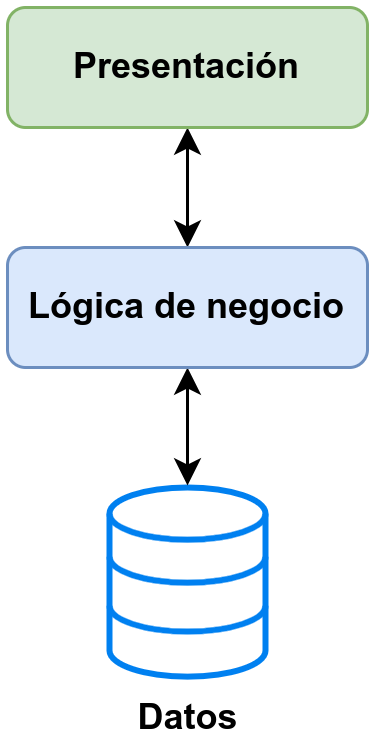
\includegraphics[width=0.25\linewidth]{capas.png}
\end{center}

\begin{itemize}
    \item \textbf{Capa de presentación}: Es la que ve el usuario (también se la denomina «capa de usuario»), presenta el sistema al usuario, le comunica la información y captura la información del usuario en un mínimo de proceso (realiza un filtrado previo para comprobar que no hay errores de formato).

    También es conocida como interfaz gráfica y debe tener la característica de ser «amigable» (entendible y fácil de usar) para el usuario. Esta capa se comunica únicamente con la capa de negocio.

    Hoy en día lo habitual es que hagamos uso de servicios web, por lo que la capa de presentación es \textbf{la web que estamos visualizando}. En el caso de aplicaciones móviles, es \textbf{la propia aplicación que tenemos instalada en el dispositivo}.

    \item \textbf{Capa de negocio}: es donde residen los programas que se ejecutan, se reciben las peticiones del usuario y se envían las respuestas tras el proceso. Se denomina capa de negocio (e incluso de lógica del negocio) porque es aquí donde se establecen todas las reglas que deben cumplirse.

    Esta capa se comunica con la capa de presentación, para recibir las solicitudes y presentar los resultados, y con la capa de datos, para solicitar al gestor de base de datos almacenar o recuperar datos de él. También se consideran aquí los programas de aplicación.

    En este tipo de arquitecturas, esta capa es la que se denomina \textbf{\textit{backend}}, y lo habitual es que sea un sistema al que llamamos a través de una \href{https://es.wikipedia.org/wiki/API}{API} (del inglés, \textit{application programming interface}, o interfaz de programación de aplicaciones).

    \item \textbf{Capa de datos}: es donde residen los datos y es la encargada de acceder a los mismos. Está formada por uno o más gestores de bases de datos que realizan todo el almacenamiento de datos, reciben solicitudes de almacenamiento o recuperación de información desde la capa de negocio.
\end{itemize}

\infobox{\textbf{Las aplicaciones web se pueden separar en dos capas: aplicación y base de datos.}}

En aplicaciones web es posible crear una arquitectura en capas aunque la aplicación no esté 100\% pensado para ello: la propia aplicación y la base de datos.


\section{Arquitectura de microservicios}

Para poder crear una \href{https://es.wikipedia.org/wiki/Arquitectura_de_microservicios}{arquitectura de microservicios} el enfoque debe darse desde el primer momento del desarrollo de software. Es decir, antes de realizar ningún tipo de programación la aplicación se planteará como pequeños servicios que podrán interactuar entre sí.


\begin{center}
    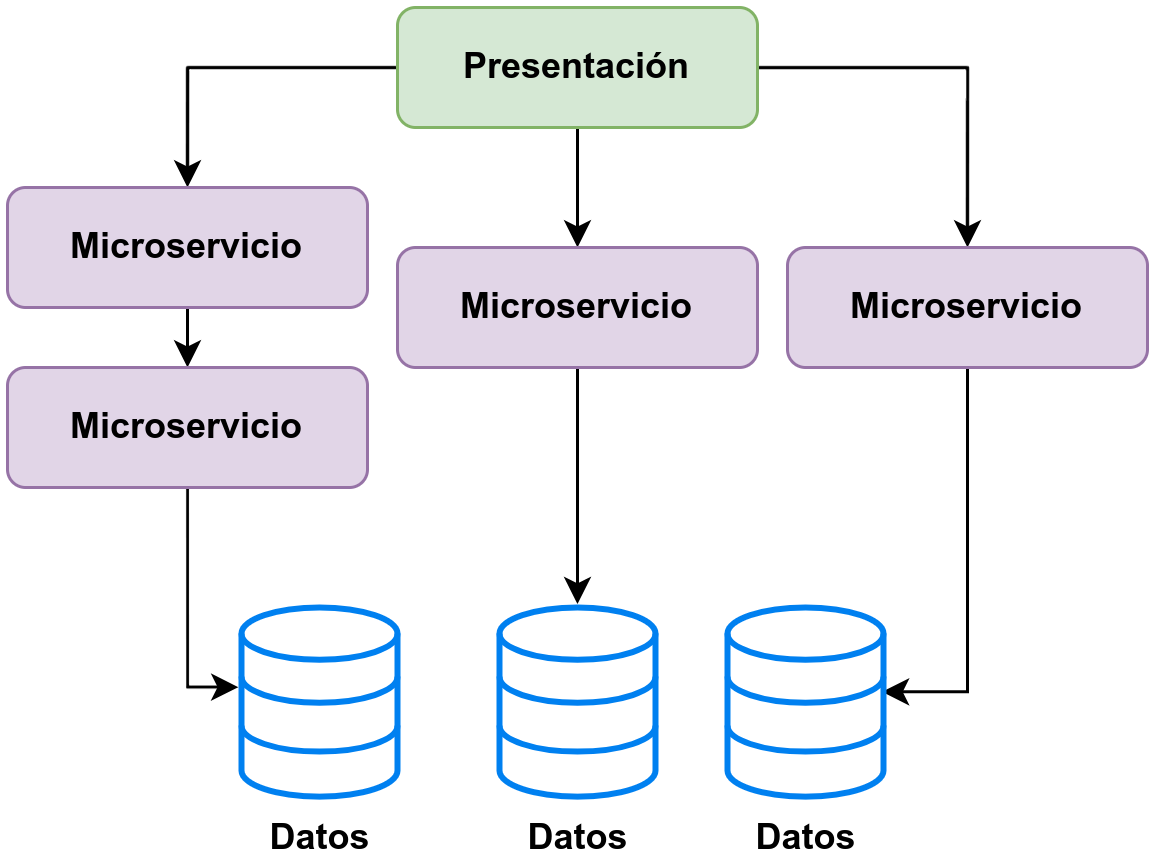
\includegraphics[width=0.7\linewidth]{microservicios.png}
\end{center}

Cada servicio se encargará de implementar una única funcionalidad. En caso de necesitar alguna característica que se repita en varios, se debería crear un microservicio que proporcione dicha característica o funcionalidad.

\infobox{\textbf{Podríamos comparar una arquitectura de microservicios como una librería de programación, en la que existen funciones que realizan una única función.}}

Cada microservicio se desplegará de manera independiente, e incluso cada uno podrá estar programado en distintos lenguajes de programación. De esta manera \textbf{se puede hacer uso del lenguaje y la tecnología más adecuada para cada funcionalidad}.



\chapter{Escalabilidad}

Teniendo en cuenta todo lo dicho hasta ahora, cuando un sistema empieza a tener problemas de rendimiento deberemos abordar el problema y plantearnos cómo solucionarlo. De no hacerlo, se corre el peligro de que el servicio se vea interrumpido y por tanto perder tiempo de trabajo.

Antes de realizar ninguna modificación habría que analizar qué es lo que está sucediendo (para ello es importante tener un buen sistema de monitorización), y de esta manera saber en qué punto existe el problema y así poder solucionarlo.

Dependiendo de las decisiones tomadas durante la instalación, y tras lo visto previamente, podremos abordarlo de dos maneras diferentes.

\infobox{“Escalabilidad” no existe en el diccionario de la \href{https://dle.rae.es/escalabilidad}{RAE}, pero se usa como anglicismo de la palabra \textbf{\textit{scalability}}.}

\section{Escalado vertical}

Cuando se escala verticalmente un sistema lo que se va a realizar es \textbf{añadir más recursos al nodo que está teniendo problemas}. Tras el análisis previo realizado se añadirán los recursos necesarios (más RAM, discos duros más rápidos, aumentar el número de procesadores/cores).

Comúnmente también se dice “meter más hierro”, porque antiguamente lo que se hacía era incrementar los recursos hardware del sistema. Hoy en día en sistemas virtualizados, estos recursos se pueden modificar, dependiendo del virtualizador, en “caliente”, por lo que no sería necesario reiniciar el servicio.

Es el sistema más simple, ya que incrementando los recursos se espera que el problema se apacigüe o desaparezca, aunque esto no tiene por qué ser siempre así.

\section{Escalado horizontal}

El escalado horizontal trata de solventar el problema repartiendo la carga entre más nodos. Este proceso de escalado es más complejo y dependerá de la modularidad del servicio ofrecido. Es decir, la lógica de la aplicación debería haberse pensado desde el inicio para un sistema que escalará de manera horizontal en el futuro.

En principio, al realizar un escalado horizontal no existe una limitación de crecimiento, ya que siempre que se pueda repartir la carga entre servidores, no importará el número de ellos.


Dentro del escalado horizontal podríamos diferenciar dos tipos:
\begin{itemize}
    \item \textbf{Escalado horizontal por capas}: Teniendo en cuenta lo visto previamente acerca de la arquitectura multicapa, en este modelo lo que se conseguirá es escalar cada capa de manera independiente. Podría realizarse de la siguiente manera:
    \begin{center}
        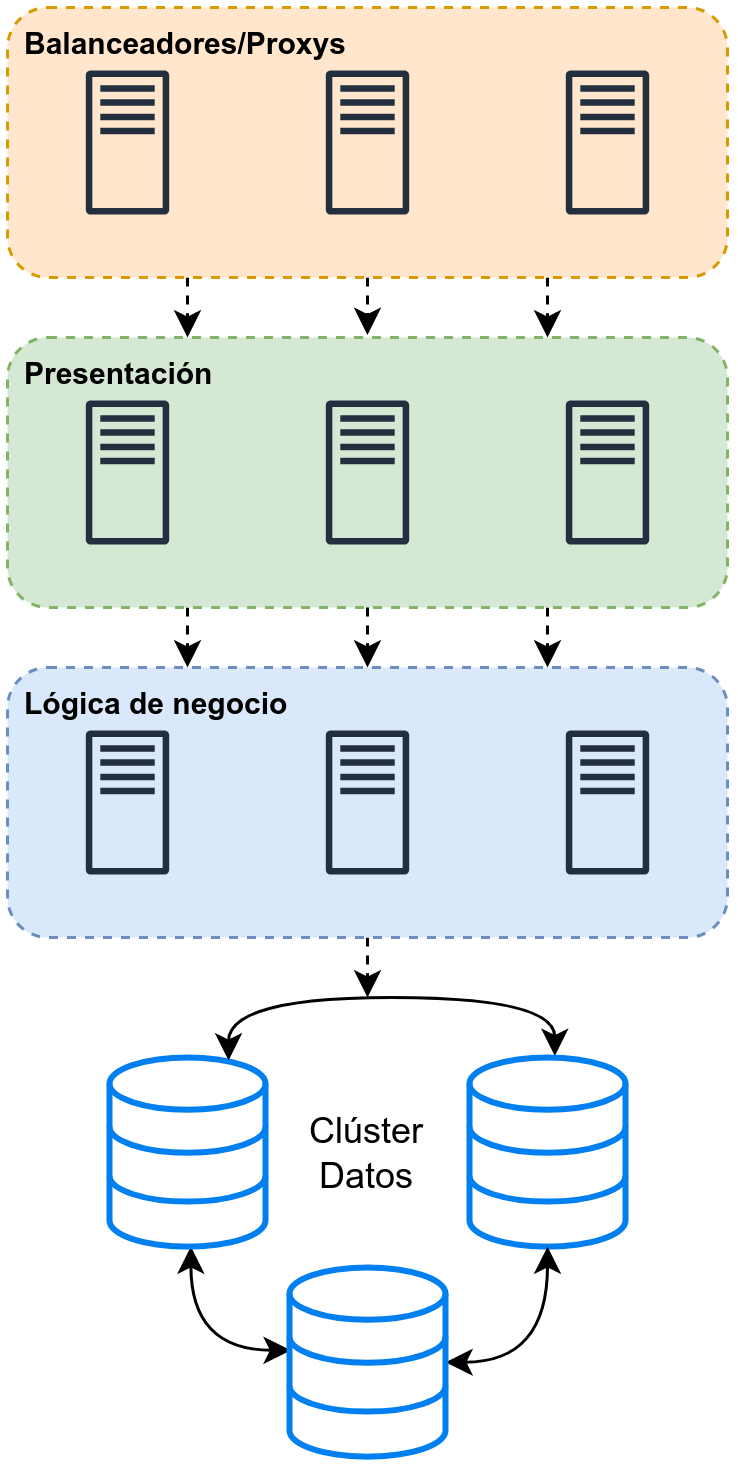
\includegraphics[width=0.4\linewidth]{capas-ha.png}
    \end{center}
    \begin{itemize}
        \item \textbf{Servidores frontales} (proxys) reciben las peticiones de la aplicación o del navegador y que balancean la carga y la mandan a servidores con la capa de presentación.
        \item Servidores con la \textbf{capa de presentación} que realizan las peticiones de negocio a los servidores correspondientes.
        \item Servidores de \textbf{lógica de negocio} que procesan las peticiones y piden los datos a un clúster de bases de datos.
        \item \textbf{Clúster de base de datos}.
    \end{itemize}

    \item \textbf{Escalado horizontal de microservicios}: En el caso del escalado de microservicios, será similar al escalado horizontal, pero en este caso sólo se escalarán los microservicios necesarios.

    Debido a que todo es mucho más modular, es posible que quizá sólo sea necesario realizar el escalado de algunos microservicios, que quizá sean los más utilizados o los que requieren más tiempo de ejecución.
\end{itemize}